% ============================================================================
% Zero-Copy Import v1.2 — technical report
% Branch: feat/zerocopy-arbitrary-cuda (f84b27c..8fafa3b)
% Build: any LaTeX with TikZ (pdflatex/xelatex/tectonic), no shell-escape.
% ============================================================================
\documentclass[11pt]{article}

\usepackage[a4paper,margin=2.6cm]{geometry}
\usepackage[T1]{fontenc}
\usepackage[utf8]{inputenc}
\usepackage{lmodern}
\usepackage{microtype}
\usepackage{amsmath}
\usepackage{booktabs}
\usepackage{xcolor}
\usepackage{tikz}
\usetikzlibrary{arrows.meta,positioning,fit,backgrounds,calc}
\usepackage{listings}
\usepackage[hidelinks]{hyperref}
\usepackage{caption}
\captionsetup{font=small,labelfont=bf}

% ---- palette -----------------------------------------------------------
\definecolor{cAppl}{HTML}{2E5E8C}   % applet side
\definecolor{cHost}{HTML}{7A4A8C}   % host side
\definecolor{cCopy}{HTML}{B03A3A}   % the copy we delete
\definecolor{cZero}{HTML}{2E7D4F}   % the zero-copy path
\definecolor{cMem}{HTML}{8C6D2E}    % memory objects
\definecolor{cInk}{HTML}{222222}

\lstset{
  basicstyle=\ttfamily\small,
  columns=fullflexible,
  keepspaces=true,
  breaklines=true,
  frame=single,
  framerule=0.3pt,
  rulecolor=\color{black!30},
  xleftmargin=0.6em,
}

\tikzset{
  box/.style   = {draw=cInk, rounded corners=2pt, align=center,
                  inner sep=5pt, minimum height=8mm, font=\small},
  mem/.style   = {box, draw=cMem, fill=cMem!8, thick},
  appl/.style  = {box, draw=cAppl, fill=cAppl!8, thick},
  host/.style  = {box, draw=cHost, fill=cHost!8, thick},
  gpu/.style   = {box, draw=cInk, fill=black!5, thick},
  flow/.style  = {-{Stealth[length=2.6mm]}, thick},
  copyflow/.style = {flow, draw=cCopy, text=cCopy},
  zeroflow/.style = {flow, draw=cZero, text=cZero},
  note/.style  = {font=\footnotesize\itshape, text=black!65, align=center},
  abiline/.style = {densely dashed, draw=black!50, thick},
}

\title{\textbf{Zero-Copy Import v1.2}\\[2pt]
\large Removing the in-VRAM copy floor for arbitrary CUDA tensors\\
in Caliper's tensor bridge}
\author{Caliper project --- branch \texttt{feat/zerocopy-arbitrary-cuda}}
\date{July 7, 2026}

\begin{document}
\maketitle

\begin{abstract}
\noindent
Caliper's tensor bridge turns live \texttt{torch} tensors into GPU textures
across a frozen C ABI. On the Vulkan/CUDA backend, an \emph{arbitrary}
framework-allocated CUDA tensor could reach a texture with zero host copies,
but never with zero copies outright: memory born in torch's caching allocator
is not exportable to Vulkan, so every texture update paid one in-VRAM
\texttt{cuMemcpyDtoD} into a host-owned interop buffer. This report describes
Bridge v1.2, which removes that floor by moving the question from
\emph{copy time} to \emph{allocation time}: an applet-side exportable memory
pool routes chosen torch allocations into \texttt{cuMemCreate} blocks carrying
shareable OS handles; the host imports each block into Vulkan \emph{once} and
runs texture updates directly from it at byte offsets. The design is additive
(no ABI break), fails closed at every gate (a refused update is a
\texttt{false} and a fallback, never a crash or a wrong image), and is
hardware-verified on an NVIDIA RTX~500~Ada (driver 596.47): byte-exact
readback tests at multiple offsets, a live training applet whose status line
reports \emph{zero-copy (imported pool)}, and an intact CPU-staged fallback
under a GL renderer. The in-VRAM copy floor is now \emph{per allocation
origin}: it persists only for memory born unshareable.
\end{abstract}

% ============================================================================
\section{Background}
% ============================================================================

Caliper hosts small ML ``applets'' behind a stable C ABI. An applet computes
with \texttt{libtorch} on whatever device it negotiated; the host renders its
UI and owns the GPU. The \emph{tensor bridge} service
(\texttt{caliper.tensor\_bridge.v1}) is the seam between the two: the applet
hands over a \texttt{CaliperTensor} descriptor, the host materializes or
updates a texture, and the applet draws it through ImGui. The v1/v1.1 headers
and dispatch tables are frozen; revisions are additive
(prefix-identical structs, new capability bits), so old applets run on new
hosts and vice versa.

Before this work the bridge had a ladder of data-crossing costs, best to
worst: \texttt{alloc\_shared} (the applet's kernels write texture-backed VRAM
in place --- literal zero-copy, but the \emph{host} chooses the allocation),
the CUDA interop path for arbitrary device tensors (zero host copies, one
in-VRAM copy), and CPU staging (the portable worst case). The middle rung is
the subject of this report.

% ============================================================================
\section{The problem: memory born unshareable}
% ============================================================================

Vulkan can read external device memory only if that memory was
\emph{allocated for export}: on Windows, a \texttt{cuMemCreate} allocation
with \texttt{CU\_MEM\_HANDLE\_TYPE\_WIN32} yields an opaque NT handle that
\texttt{vkAllocateMemory} can import. Memory obtained from plain
\texttt{cudaMalloc} --- which is what torch's caching allocator uses ---
carries no such handle and cannot be retrofitted with one. Exportability is
decided at \emph{allocation time}, by allocation \emph{flags}.

Consequently, for an arbitrary torch CUDA tensor the host can do no better
than: keep a host-owned, exportable interop buffer behind each texture, and
on every update copy the tensor's bytes into it with \texttt{cuMemcpyDtoD}
(Figure~\ref{fig:before}). The copy is device-to-device and cheap in absolute
terms, but it is paid \emph{per update, forever}, it doubles the working-set
touch for large maps, and it is a standing asterisk on the platform's
zero-copy story: the whitepaper had to state a ``one in-VRAM-copy floor'' for
framework-allocated tensors.

\begin{figure}[ht]
\centering
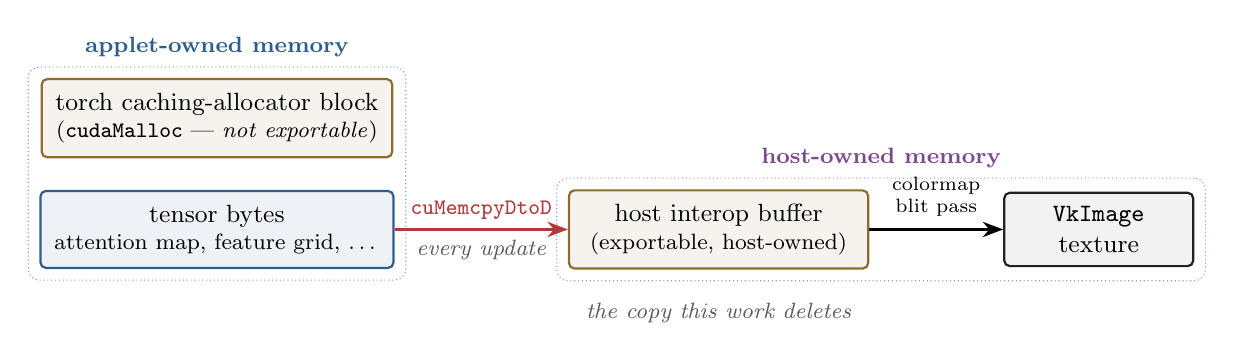
\begin{tikzpicture}[node distance=7mm and 12mm]
  % applet side
  \node[mem, minimum width=42mm] (blk)
    {torch caching-allocator block\\[-1pt]
     {\footnotesize (\texttt{cudaMalloc} --- \emph{not exportable})}};
  \node[appl, below=4mm of blk, minimum width=42mm] (tensor)
    {tensor bytes\\[-1pt] {\footnotesize attention map, feature grid, \dots}};
  % host side
  \node[mem, right=22mm of tensor, minimum width=38mm] (interop)
    {host interop buffer\\[-1pt]
     {\footnotesize (exportable, host-owned)}};
  \node[gpu, right=17mm of interop, minimum width=24mm] (tex)
    {\texttt{VkImage}\\ texture};
  % flows
  \draw[copyflow] (tensor) -- node[above, font=\footnotesize\bfseries]
    {\texttt{cuMemcpyDtoD}} node[below, note] {every update} (interop);
  \draw[flow] (interop) -- node[above=1pt, font=\scriptsize, align=center]
    {colormap\\ blit pass} (tex);
  % brace note
  \node[note, below=3mm of interop] {the copy this work deletes};
  \begin{scope}[on background layer]
    \node[fit=(blk)(tensor), draw=cAppl!60, densely dotted, rounded corners,
          inner sep=4pt, label={[cAppl,font=\footnotesize\bfseries]above:applet-owned memory}] {};
    \node[fit=(interop)(tex), draw=cHost!60, densely dotted, rounded corners,
          inner sep=4pt, label={[cHost,font=\footnotesize\bfseries]above:host-owned memory}] {};
  \end{scope}
\end{tikzpicture}
\caption{The v1 interop path for an arbitrary CUDA tensor. The tensor's
memory cannot be imported by Vulkan, so its bytes are copied in VRAM into a
host-owned exportable buffer on \emph{every} texture update --- the
``in-VRAM copy floor.''}
\label{fig:before}
\end{figure}

Two constraints rule out the obvious dodges. The host cannot simply allocate
all applet tensors itself (\texttt{alloc\_shared} exists, but forcing every
intermediate through host allocations would invert ownership of the applet's
compute). And the ABI cannot change shape: v1/v1.1 applets must keep working
bit-for-bit.

% ============================================================================
\section{The idea: change where memory is born}
% ============================================================================

If exportability is decided at allocation time, then the fix belongs at
allocation time. Torch 2.5 provides the two hooks needed to apply it
\emph{selectively}, from the applet side, without forking torch:

\begin{enumerate}
  \item \texttt{CUDAPluggableAllocator} --- user-supplied alloc and free
        hooks behind torch's caching allocator; and
  \item \texttt{c10::cuda::MemPool} + \texttt{beginAllocateToPool} --- a
        scope that routes the allocations made \emph{inside it} to a chosen
        pool (the mechanism CUDA graphs use).
\end{enumerate}

\noindent
The SDK's new \texttt{ExportablePool} combines them: its allocation function
builds blocks with \texttt{cuMemCreate} (+\,\texttt{WIN32} shareable handle
type), maps them with \texttt{cuMemMap}/\texttt{cuMemSetAccess}, exports the
OS handle, and registers the block in an interval map
(\texttt{AllocRegistry}: pointer $\rightarrow$ (block, byte offset)). An
applet materializes exactly the tensors it wants to display inside
\texttt{pool.use()}; everything else in the process keeps torch's default
allocator. The host imports each block \emph{once} and thereafter updates
textures straight out of it (Figure~\ref{fig:after}).

\begin{figure}[ht]
\centering
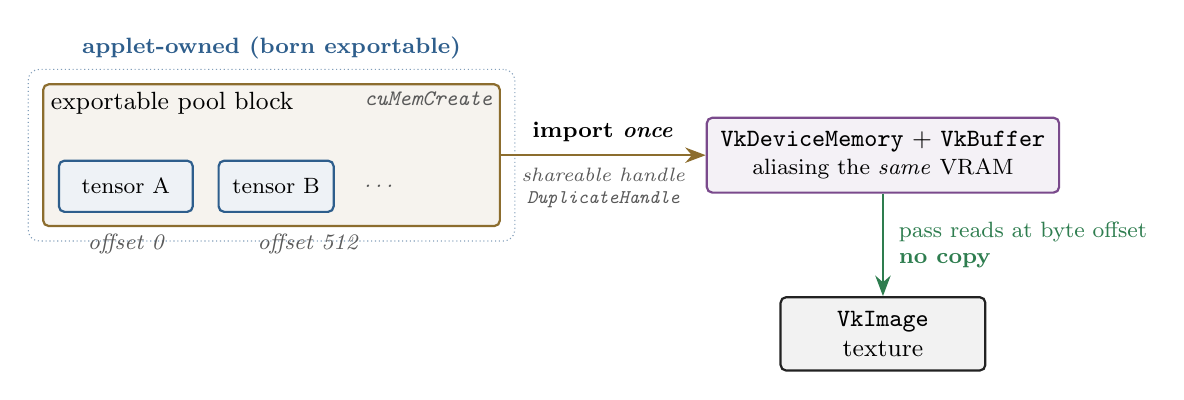
\begin{tikzpicture}[node distance=7mm and 12mm]
  % the pool block with tensors at offsets
  \node[mem, minimum width=58mm, minimum height=18mm] (blk) {};
  \node[font=\small, anchor=north west, inner sep=3pt] at (blk.north west)
    {exportable pool block};
  \node[note, anchor=north east, inner sep=3pt] at (blk.north east)
    {\texttt{cuMemCreate}};
  \node[appl, minimum width=17mm, minimum height=6.5mm, anchor=south west,
        font=\footnotesize] at ($(blk.south west)+(2mm,1.8mm)$) (t0) {tensor A};
  \node[appl, minimum width=13mm, minimum height=6.5mm, right=3mm of t0,
        font=\footnotesize] (t1) {tensor B};
  \node[note, right=2.5mm of t1] {\dots};
  \node[note, anchor=north] at ($(t0.south)+(0,-1.5mm)$) {offset 0};
  \node[note, anchor=north] at ($(t1.south)+(4mm,-1.5mm)$) {offset 512};
  % host side
  \node[host, right=26mm of blk, minimum width=38mm] (vkmem)
    {\texttt{VkDeviceMemory} + \texttt{VkBuffer}\\[-1pt]
     {\footnotesize aliasing the \emph{same} VRAM}};
  \node[gpu, below=13mm of vkmem, minimum width=26mm] (tex)
    {\texttt{VkImage}\\ texture};
  % flows
  \draw[flow, draw=cMem] (blk) -- node[above=1pt, font=\footnotesize\bfseries]
    {import \emph{once}} node[below=1pt, font=\scriptsize\itshape,
    text=black!65, align=center]
    {shareable handle\\ \texttt{DuplicateHandle}} (vkmem);
  \draw[zeroflow] (vkmem) -- node[right=2pt, font=\footnotesize, align=left]
    {pass reads at byte offset\\ \textbf{no copy}} (tex);
  \begin{scope}[on background layer]
    \node[fit=(blk)(t0)(t1), draw=cAppl!60, densely dotted, rounded corners,
          inner sep=5pt,
          label={[cAppl,font=\footnotesize\bfseries]above:applet-owned (born exportable)}] {};
  \end{scope}
\end{tikzpicture}
\caption{The v1.2 imported path. The pool block is imported into Vulkan once;
every tensor inside it is addressed by byte offset, and the colormap/blit
pass reads the tensor's bytes \emph{in place}. The per-update
\texttt{cuMemcpyDtoD} of Figure~\ref{fig:before} no longer exists. (Blocks
are 2\,MiB-granularity \texttt{cuMemCreate} allocations; torch sub-allocates
tensors at 512-byte alignment.)}
\label{fig:after}
\end{figure}

The floor therefore becomes a statement about \emph{origin}, not about
frameworks: tensors born in the pool update with zero copies of their data;
tensors born unshareable (default torch allocator, any foreign allocator)
keep the one-copy interop path, unchanged.

% ============================================================================
\section{Architecture}
% ============================================================================

Figure~\ref{fig:arch} shows the pieces and who owns them. The ABI grows by
one additive revision, \texttt{caliper.tensor\_bridge.v1\_2}: the same seven
members as v1.1, prefix-identical, plus three entry points and one
capability bit.

\begin{lstlisting}
/* caps() bit 1: the host can import applet-exported allocations. */
#define CALIPER_BRIDGE_CAP_IMPORT_ALLOC (1u << 1)

CaliperAllocId import_allocation(void* os_handle, uint64_t size_bytes,
                                 uint32_t handle_type);   /* 0 = declined */
void           release_allocation(CaliperAllocId alloc);
bool           update_texture_from_alloc(CaliperTextureId tex,
                                         CaliperAllocId alloc,
                                         uint64_t offset_bytes,
                                         const CaliperTensor* desc);
\end{lstlisting}

\noindent
\texttt{desc} carries shape/dtype/strides/stream; its \texttt{data} pointer
is ignored --- the (allocation, offset) pair \emph{is} the address. The header
also states the memory-stability contract: the pass reads the imported bytes
in place, so the window $[\text{offset}, \text{offset}+\text{extent})$ must
not be rewritten until the texture's next update.

\begin{figure}[ht]
\centering
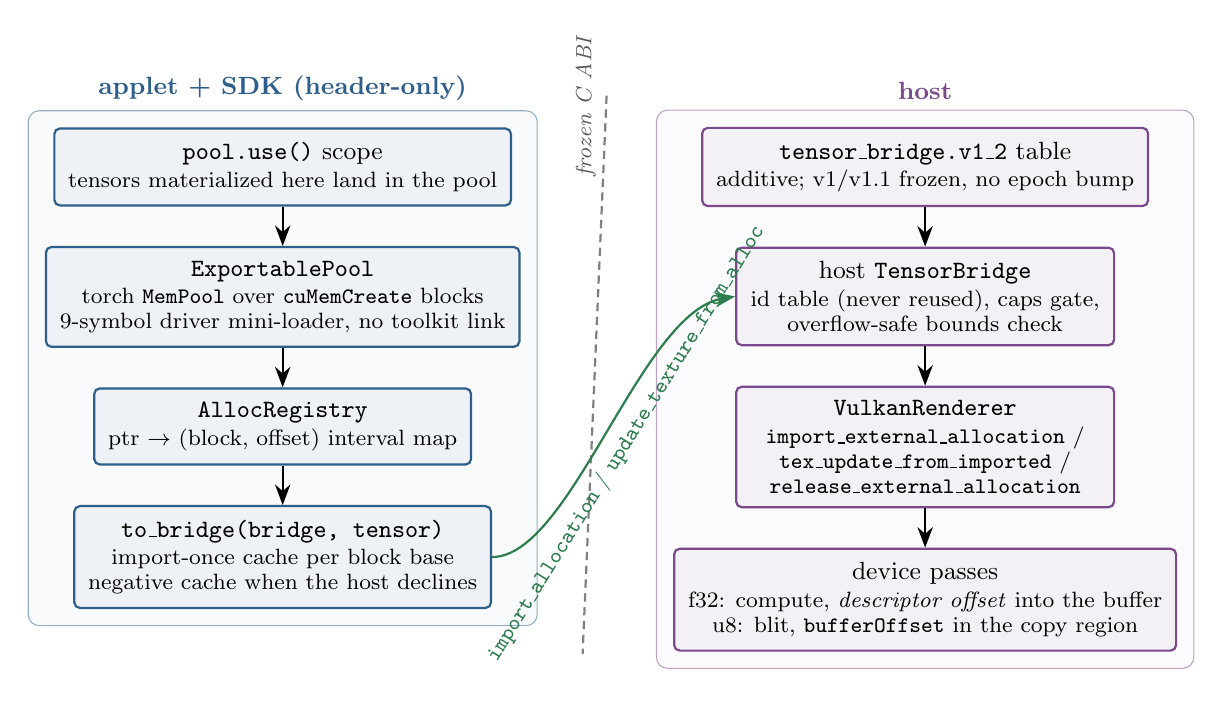
\begin{tikzpicture}[node distance=5mm and 8mm]
  % ---- applet column ----
  \node[appl, minimum width=46mm] (uscope)
    {\texttt{pool.use()} scope\\[-1pt]
     {\footnotesize tensors materialized here land in the pool}};
  \node[appl, below=of uscope, minimum width=46mm] (pool)
    {\texttt{ExportablePool}\\[-1pt]
     {\footnotesize torch \texttt{MemPool} over \texttt{cuMemCreate} blocks}\\[-2pt]
     {\footnotesize 9-symbol driver mini-loader, no toolkit link}};
  \node[appl, below=of pool, minimum width=46mm] (reg)
    {\texttt{AllocRegistry}\\[-1pt]
     {\footnotesize ptr $\rightarrow$ (block, offset) interval map}};
  \node[appl, below=of reg, minimum width=46mm] (tobridge)
    {\texttt{to\_bridge(bridge, tensor)}\\[-1pt]
     {\footnotesize import-once cache per block base}\\[-2pt]
     {\footnotesize negative cache when the host declines}};
  % ---- host column ----
  \node[host, right=24mm of uscope, minimum width=48mm] (table)
    {\texttt{tensor\_bridge.v1\_2} table\\[-1pt]
     {\footnotesize additive; v1/v1.1 frozen, no epoch bump}};
  \node[host, below=of table, minimum width=48mm] (tb)
    {host \texttt{TensorBridge}\\[-1pt]
     {\footnotesize id table (never reused), caps gate,}\\[-2pt]
     {\footnotesize overflow-safe bounds check}};
  \node[host, below=of tb, minimum width=48mm] (vk)
    {\texttt{VulkanRenderer}\\[-1pt]
     {\footnotesize \texttt{import\_external\_allocation} /}\\[-2pt]
     {\footnotesize \texttt{tex\_update\_from\_imported} /}\\[-2pt]
     {\footnotesize \texttt{release\_external\_allocation}}};
  \node[host, below=of vk, minimum width=48mm] (paths)
    {device passes\\[-1pt]
     {\footnotesize f32: compute, \emph{descriptor offset} into the buffer}\\[-2pt]
     {\footnotesize u8: blit, \texttt{bufferOffset} in the copy region}};
  % ---- ABI line ----
  \draw[abiline] ($(uscope.north east)!0.5!(table.north west)+(0,4mm)$)
              -- ($(tobridge.south east)!0.5!(paths.south west)-(0,3mm)$)
     node[pos=0.02, note, rotate=90, anchor=south] {frozen C ABI};
  % ---- cross arrows ----
  \draw[flow] (uscope) -- (pool);
  \draw[flow] (pool) -- (reg);
  \draw[flow] (reg) -- (tobridge);
  \draw[flow] (table) -- (tb);
  \draw[flow] (tb) -- (vk);
  \draw[flow] (vk) -- (paths);
  \draw[zeroflow] (tobridge.east) .. controls +(10mm,0) and +(-12mm,-2mm) ..
    node[below, sloped, font=\footnotesize]
    {\texttt{import\_allocation} / \texttt{update\_texture\_from\_alloc}}
    (tb.west);
  \begin{scope}[on background layer]
    \node[fit=(uscope)(pool)(reg)(tobridge), draw=cAppl!50, rounded corners,
          inner sep=6pt, fill=cAppl!3,
          label={[cAppl,font=\small\bfseries]above:applet + SDK (header-only)}] {};
    \node[fit=(table)(tb)(vk)(paths), draw=cHost!50, rounded corners,
          inner sep=6pt, fill=cHost!3,
          label={[cHost,font=\small\bfseries]above:host}] {};
  \end{scope}
\end{tikzpicture}
\caption{Component view. The SDK side is header-only and loads its nine
\texttt{cuMem*} driver symbols itself (no CUDA toolkit link, per the
platform's dependency rules); the host side is one additive dispatch table
over existing renderer seams. Import happens once per block and is cached by
block base address on the applet side.}
\label{fig:arch}
\end{figure}

\subsection{The update path}
For an f32 mapped texture the colormap compute pass binds the imported
\texttt{VkBuffer} with a \emph{descriptor offset} equal to the tensor's byte
offset --- the shader is unchanged and never knows it is reading foreign
memory. For u8 RGBA the blit path sets \texttt{bufferOffset} in the
buffer-to-image copy region. Both device paths report distinct telemetry
(\texttt{"compute-imported"} / \texttt{"blit-imported"}) so tests and status
lines can claim exactly the path that ran. Synchronization reuses the
existing V4 machinery: the pipelined chain signals the shared timeline
semaphore \emph{without} a preceding copy, and where timeline semaphores are
unavailable the fenced synchronous fallback applies.

\subsection{Failing closed}
Every gate refuses by returning \texttt{false} or \texttt{0}, leaving pixels
and telemetry untouched; the caller falls through to the copying path. Gates
include: capability bit absent; handle import failure (unwound completely);
offset misaligned for the f32 descriptor-offset path --- the Vulkan
\texttt{minStorageBuffer\-OffsetAlignment} limit; torch sub-allocations are
512-aligned, so real pool tensors pass; window out of bounds, checked
overflow-safely at \emph{both} the bridge and the renderer, phrased as
\mbox{\texttt{offset > size}} \texttt{||} \mbox{\texttt{bytes > size -
offset}} so no sum can wrap; allocation already released (ids are never
reused); and a buffer whose memory requirements exceed the imported size
(logged, declined). A failed import is never a crash and never a wrong
image.

\subsection{Lifetime}
Block frees are initiated by torch's allocator, which may run its callback
on any thread; the bridge, by contract, is frame-thread-only. The pool
therefore \emph{queues} host-import releases in the free callback and drains
the queue at its two frame-thread call sites (\texttt{to\_bridge} and the
destructor). The destructor additionally releases the import of every block
it reclaims itself, so correctness does not depend on whether torch's
\texttt{releasePool} frees cached segments synchronously. The exemplar applet
guards the last edge: if its worker outlives the shutdown cancel grace, the
pool is deliberately leaked (with a log line) rather than destroyed under a
live worker --- a leak at process exit, never a use-after-free.

% ============================================================================
\section{The exemplar: \texttt{gpt\_scope}}
% ============================================================================

\texttt{gpt\_scope} trains a small character transformer and shows a
per-head attention heatmap. It opts in lazily: on the first CUDA probe, if
the host grants \texttt{IMPORT\_ALLOC} and torch reports CUDA, it constructs
one \texttt{ExportablePool}; on any failure the pool stays null and the
applet is byte-identical to its pre-v1.2 self.

Two realities of the existing code shaped the integration. First, the tensor
actually uploaded is not the raw attention snapshot but a block-upscaled
derivative built at the upload site --- so in pool mode the \emph{worker}
materializes the per-head upscaled tensors inside \texttt{pool.use()} (the
worker is the only thread allocating CUDA memory during that scope, which
keeps foreign allocations out of the pool). Second, a mapped texture's
value range is fixed at creation, and per-head ranges differ --- which is
precisely why the old code re-created the texture on every selection change.
Pool mode instead pre-normalizes each head by its own maximum into a fixed
$[0,1]$ mapping, so one texture is created once and every subsequent
probe/selection change is an \emph{update} --- the operation the imported
path accelerates. The heatmap status line says
\emph{``zero-copy (imported pool)''} only while the displayed texture's
latest content actually arrived through \texttt{update\_texture\_from\_alloc}
(the platform reserves ``zero-copy'' wording for paths that literally are).

% ============================================================================
\section{Verification}
% ============================================================================

All results below were produced on the target machine: Windows~11, NVIDIA
RTX~500~Ada (laptop), driver 596.47, Vulkan renderer, torch/libtorch 2.5.1
CUDA~12.1.

\subsection{Byte-exact test rows}
Five hardware-gated rows were added to the gfx suite, each driving a real
\texttt{cuMemCreate} block through the public ABI (the host gained a separate
\emph{optional} \texttt{VmmApi} driver table so tests can build shareable
allocations; the core driver table's all-or-nothing rule is untouched).
``Byte-exact'' is literal: \texttt{==} on the RGBA8 readback against the CPU
reference, no tolerances.

\begin{table}[ht]
\centering\footnotesize
\begin{tabular}{@{}lll@{}}
\toprule
Row & Exercises & Expectation \\
\midrule
f32 at offsets 0 and 512 & descriptor-offset compute &
  \texttt{"compute-imported"}, byte-exact at 0 and 512 \\
misaligned offset 4 & alignment gate &
  \texttt{false}; pixels and telemetry untouched \\
u8 RGBA at offset 512 & blit \texttt{bufferOffset} &
  \texttt{"blit-imported"}, byte-exact; 3-channel \texttt{false} \\
release + reuse & id lifecycle &
  update-after-release \texttt{false}; 50$\times$ import/release, \\
  & & ids strictly increasing \\
out-of-bounds window & both bounds gates &
  \texttt{false} for past-end and straddling windows \\
\bottomrule
\end{tabular}
\caption{The five imported-allocation rows. Full suite after integration:
22 cases, 1030 assertions, green; the pre-existing CUDA rows (device
compute path, \texttt{alloc\_shared}, burst pipelining) prove the
refactoring left the donor paths byte-identical.}
\label{tab:rows}
\end{table}

\subsection{Live application}
A live \texttt{gpt\_scope} session on the Vulkan renderer: training on CUDA,
with the renderer logging \emph{``import path OK --- zero-copy (imported
allocation in place)''} on the first imported update, status line
\emph{``zero-copy (imported pool)''} (screenshot-verified at training step
344), head-selection switching through the update path, cancel and relaunch
mid-run clean, and a mid-run applet unload driving the pool destructor with
live imports --- no crashes, no validation errors, no frame-watchdog stalls.
Under \texttt{CALIPER\_RENDERER=gl} the same applet trains and renders
identically via CPU staging (the log shows the expected foreign-device
rejection), demonstrating the fallback intact.

\subsection{Findings worth recording}
Three defects were found and fixed \emph{only because} the code first ran on
real hardware, and one was a specification bug:

\begin{itemize}
  \item \textbf{\texttt{SECURITY\_ATTRIBUTES} required.} On this driver, a
        WIN32-shareable \texttt{cuMemCreate} carrying a null
        \texttt{win32HandleMetaData} returns
        \texttt{CUDA\_ERROR\_INVALID\_VALUE} (surfaced, confusingly, as a
        torch ``OOM''). An exportable NT handle needs security attributes
        --- the CUDA \texttt{memMapIPCDrv} sample's precedent.
  \item \textbf{Cold-start ordering.} \texttt{beginAllocateToPool} before
        torch's lazy CUDA initialization terminates the process; the pool
        constructor now forces \texttt{lazyInitCUDA()}.
  \item \textbf{Spec geometry bug.} The handoff's first test row specified a
        $17{\times}9$ f32 grid at offset 0 \emph{and} a second grid at
        offset 512 --- but $17{\times}9{\times}4 = 612 > 512$: the regions
        overlap, and the renderer honestly rendered the clobbered bytes
        while the reference assumed pristine data. The row now writes,
        updates, and verifies each region in sequence. The failure mode
        (first divergent byte exactly at output byte 512) is a small
        advertisement for byte-exact assertions.
  \item \textbf{Review-found lifetime bugs.} A final whole-branch review
        surfaced the release-ordering and threading issues summarized in
        the Lifetime section; all were fixed and re-verified before this
        report.
\end{itemize}

% ============================================================================
\section{Limits and non-claims}
% ============================================================================

\begin{itemize}
  \item The floor is removed only for memory born in the exportable pool;
        default-allocator and foreign-allocator tensors keep the one-copy
        interop path. This is inherent, not incidental: exportability is an
        allocation-time property.
  \item Hardware verification covers Windows + NVIDIA + Vulkan. The POSIX
        file-descriptor handle path is stubbed and inert; Linux import is a
        port task, not a claim.
  \item In pool mode the exemplar pre-normalizes attention values in f32
        before the shader maps them; against the old path this can differ by
        at most one 8-bit quantization step. The cap-absent path is
        byte-identical to the pre-v1.2 applet.
  \item The imported bytes must stay stable between an update and the
        texture's next update; the ABI documents this, and at the exemplar's
        probe cadence the window is negligible, but a pathological producer
        could violate it.
\end{itemize}

% ============================================================================
\section{Conclusion}
% ============================================================================

The interesting move was recognizing that ``arbitrary tensors cost one copy''
was never a statement about tensors --- it was a statement about where their
memory was born. Torch's pluggable-allocator machinery lets an applet change
that birthplace for exactly the tensors it wants to display, and one
imported block then serves unlimited zero-copy texture updates at byte
offsets. Everything else in the design --- the additive ABI, the two-layer
bounds checks, the fail-closed ladder, the wording discipline --- exists to
make that one move safe to ship on a frozen platform. The floor still exists;
it just moved to where it belongs: on memory that genuinely cannot be shared.

\end{document}
